\tikzset{fontscale/.style = {font=\relsize{#1}}
    }
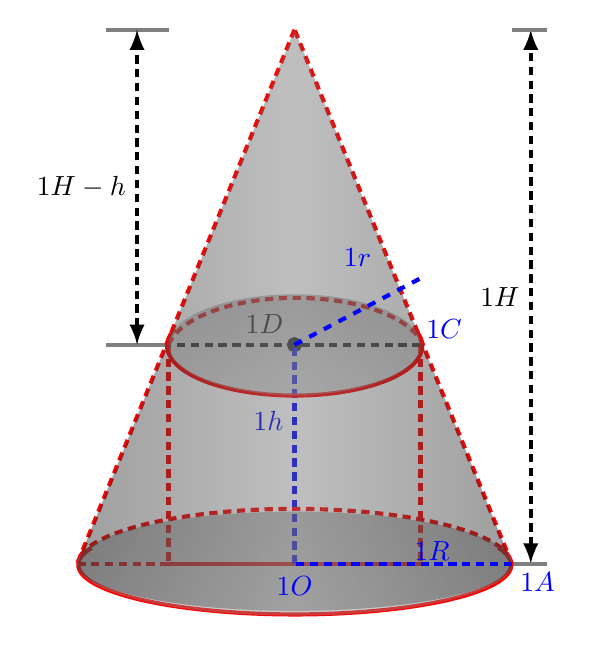
\begin{tikzpicture}[font = \sansmath,fontscale=1,scale=2,line width=1.5pt]
%\draw [very thin, style=gray!50, step=0.5] (-3,-2) grid (3,2);
  \coordinate (O) at (0,0);
 \coordinate (A) at (-1.38,1.39);
 \coordinate (B) at (-1.38,-1.39);
 \coordinate (C) at (1.38,1.39);
 \coordinate (D) at (1.38,-1.39);
\coordinate (E) at (0,-1.39);
\coordinate (F) at (0,2);
\coordinate (G) at (1.5,-1.39);
\coordinate (H) at (1.5,2);
\coordinate (I) at (-0.8,0);
\coordinate (J) at (0.8,0);
\draw[color=blue] (J) node[above right=-2pt] {$C$};
   
 \draw[densely dashed,latex-latex] (G) to [edge label = $H$] (H);
 \draw[gray] (D) to (1.6,-1.39);
 \draw[gray] (1.38,2) to (1.6,2);
\draw[gray] (-0.8,0) to (-1.2,0);
\draw[gray] (-0.8,2) to (-1.2,2);
 \draw[densely dashed,latex-latex] (-1,0) to [edge label = $H-h$] (-1,2);
\draw[densely dashed,red] (B) to(E);
\draw[densely dashed,red] (I) to(-0.8,-1.39);
\draw[densely dashed,red] (J) to(0.8,-1.39);
 \draw[densely dashed] (J) to  (I);
\draw[red] (0.8,-1.39) to(-0.8,-1.39);
% label of ball center point
  \filldraw (O) circle (1pt) node[above left] {$D$};

%cilindro
 \draw[densely dashed,red] (D) to (F);
\draw[densely dashed,red] (F) to (B);

\draw[densely dashed,blue] (E) to [above=12pt,edge label = $h$] (O);

  % cut of ball surface botton
%  
  \draw[red, densely dashed] (-1.36,-1.34) arc [start angle = 170, end angle = 10,
    x radius = 13.8mm, y radius = 3.6mm];
  \draw[red] (-1.29,-1.29) arc [start angle=-200, end angle = 20,
    x radius = 13.75mm, y radius = 3.15mm];

%centro of ball 
 \draw[red, densely dashed] (-0.8,0) arc [start angle = 170, end angle = 10,
    x radius = 8.2mm, y radius = 3.6mm];
  \draw[red] (-0.76,0.1) arc [start angle=-200, end angle = 20,
    x radius = 8.1mm, y radius = 3.15mm];
\fill[
  top color=gray!50,
  bottom color=gray!10,
  shading=axis,
  opacity=0.25
  ] 
  (0,-1.39) circle (1.38cm and 0.33cm);
\fill[
  left color=gray!50!black,
  right color=gray!50!black,
  middle color=gray!50,
  shading=axis,
  opacity=0.25
  ] 
  (1.38,-1.39) -- (0,2) -- (-1.38,-1.39) arc (180:360:1.38cm and 0.3cm);
%%%%%%%%%%%%%%%%%%%%%
\fill[
  top color=gray!50,
  bottom color=gray!10,
  shading=axis,
  opacity=0.25
  ] 
  (0,0) circle (0.8cm and 0.32cm);
%%%%%%%%%%%%%%%%%%%%%5
\draw[densely dashed,blue] (D) to [above=12pt,edge label = $R$] (E);
\draw[dashed,blue] (O) to [above=12pt,edge label = $r$] (0.8,0);
\draw[color=blue] (0,-1.38) node[below =1pt] {$O$};
\draw[color=blue] (D) node[below right =-1pt] {$A$};

\end{tikzpicture}
